\chapter{Implementation}

\section{Introduction}
This chapter covers the technical realization of Sila DZ. It details the software technologies, development tools, and the microservices architecture that power the platform. Furthermore, we break down the application into distinct functional parts to explain the implementation logic accompanied by visual interfaces.

\section{Software Technologies}

\subsection{Frontend Technologies}
\begin{itemize}
    \item \textbf{React.js:} A declarative, efficient, and flexible JavaScript library for building user interfaces. We utilized React alongside Vite to build a fast, single-page web application (SPA) for the Web Dashboard and Admin Panel.
    \item \textbf{Flutter:} An open-source UI software development kit created by Google. Flutter was used to develop the cross-platform mobile application, allowing us to compile native code for both Android and iOS from a single Dart codebase.
\end{itemize}

\subsection{Backend Technologies}
\begin{itemize}
    \item \textbf{Spring Boot:} A Java-based framework used to create stand-alone, production-grade Spring applications. We utilized Spring Boot to implement our core Microservices Architecture, specifically serving as the \textbf{API Gateway} (routing traffic) and the \textbf{Service Registry} (Eureka) for service discovery.
    \item \textbf{NestJS \& Node.js:} NestJS is a progressive Node.js framework for building efficient and scalable server-side applications. We used NestJS and Express (Node.js) to build specialized microservices that handle real-time I/O operations, such as the negotiation chat and notifications.
\end{itemize}

\subsection{Infrastructure and Data Management}
\begin{itemize}
    \item \textbf{Apache Kafka:} Integrated as our message broker, Kafka ensures reliable, asynchronous communication between our Spring Boot and Node.js microservices.
    \item \textbf{PostgreSQL:} Used as our primary relational database for strict transactional data, such as user balances, order states, and payment records.
    \item \textbf{MongoDB:} Deployed as our NoSQL database to store flexible, document-based data such as chat messages histories and dynamic user session logs.
\end{itemize}

\subsection{Development Tools}
\begin{itemize}
    \item \textbf{Visual Studio Code (VS Code):} The primary lightweight IDE used for developing the React frontend, Flutter mobile app, and Node.js microservices.
    \item \textbf{IntelliJ IDEA:} A powerful Java IDE used exclusively for developing, debugging, and managing the Spring Boot microservices ecosystem.
\end{itemize}

\section{System Architecture and Deployment}
The backend architecture is fully decentralized. The \textbf{Spring Cloud Gateway} receives all incoming HTTP and WebSocket traffic from the React web app and Flutter mobile app. It then consults the \textbf{Service Registry} to route requests to the appropriate underlying microservice (e.g., Auth Service, Order Service, Chat Service). When an order is placed, the Order Service publishes an event to \textbf{Kafka}, which is then consumed by the Notification Service (Node.js) to push a real-time update to the client via \textbf{SSE} or WebSockets. The entire infrastructure is containerized using Docker to ensure seamless deployment and scalability in cloud environments.

\section{Implementation of Core Modules}

\subsection{Order Management Module}
The Order Management module is the heart of Sila DZ. Importers can view incoming requests, while clients can track their packages. The frontend consumes RESTful APIs from the Order Microservice, fetching data in real-time. The interface utilizes a responsive Grid layout, ensuring that order statuses are color-coded and clearly visible.

% =========== ORDER MANAGEMENT SCREENSHOT ===========
\begin{figure}[H]
    \centering
    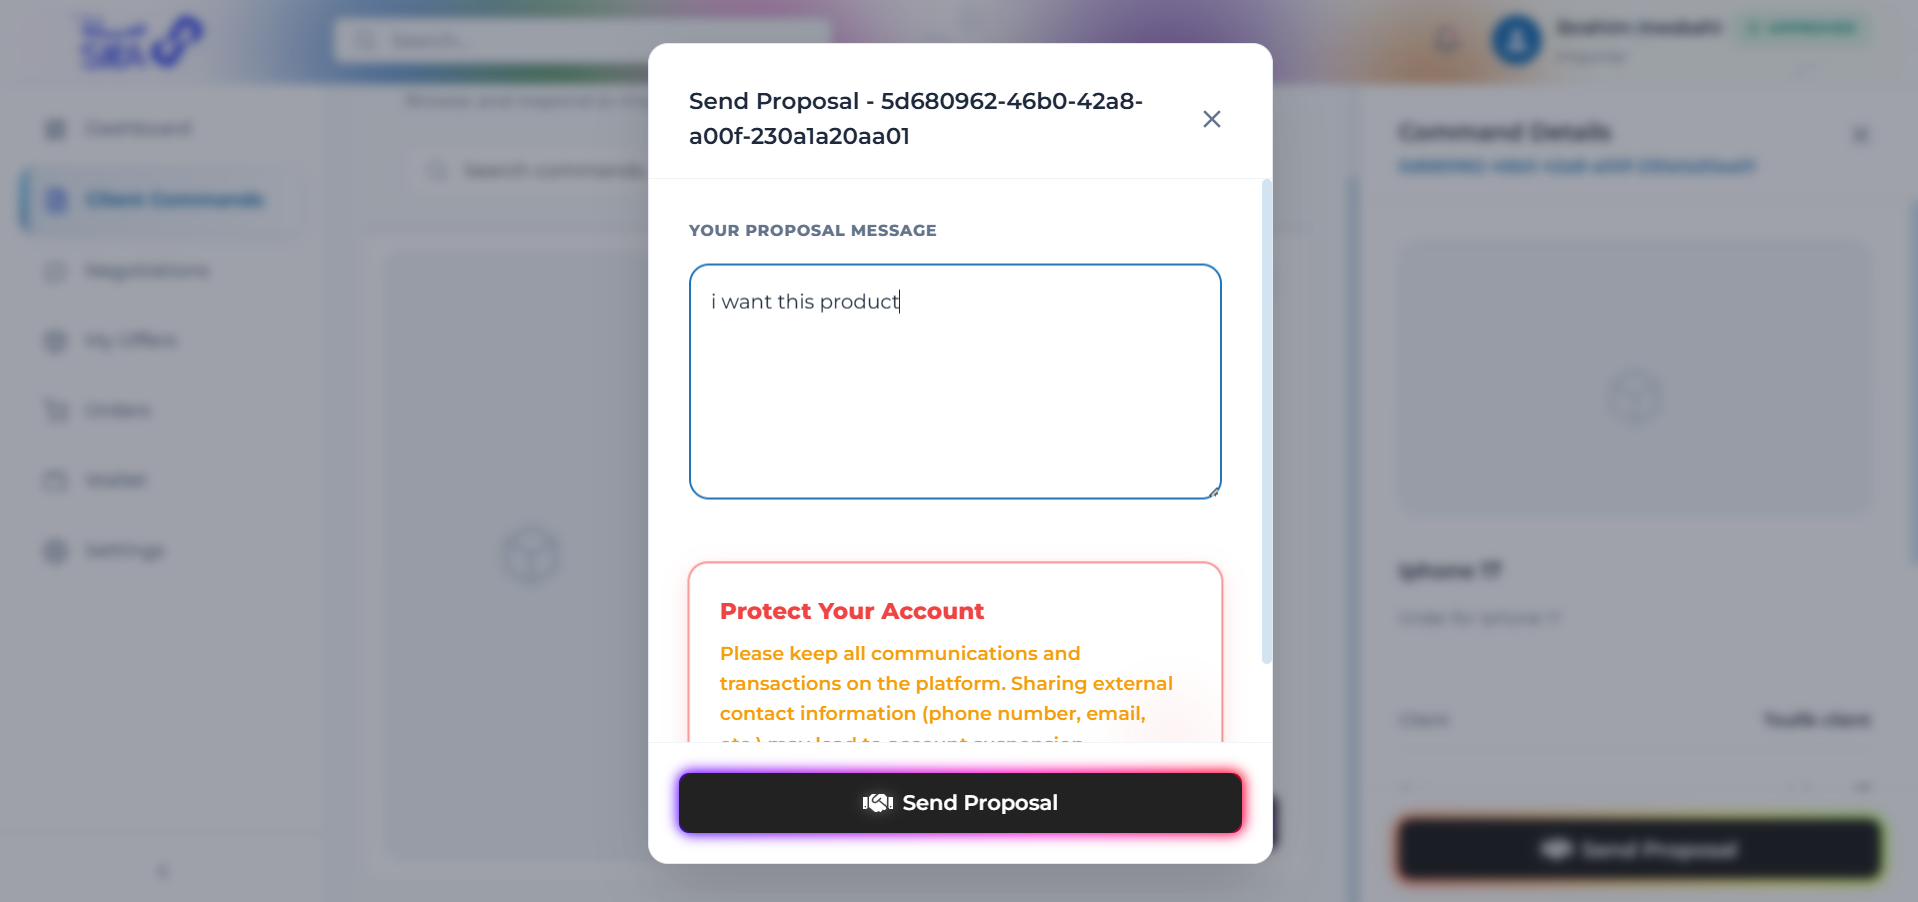
\includegraphics[width=0.9\textwidth]{assets/CMD-Proposal.png}
    \caption{Order Management Dashboard Interface}
    \label{fig:order_management}
\end{figure}
% ===============================================================

\subsection{Real-time Negotiation Module}
To eliminate informal haggling, we built a dedicated negotiation room. This module leverages WebSockets connected to a NestJS microservice. It allows clients to send counter-offers and importers to accept them instantly. The chat history is persisted in MongoDB for fast retrieval.

% =========== NEGOTIATION SCREENSHOT ===========
\begin{figure}[H]
    \centering
    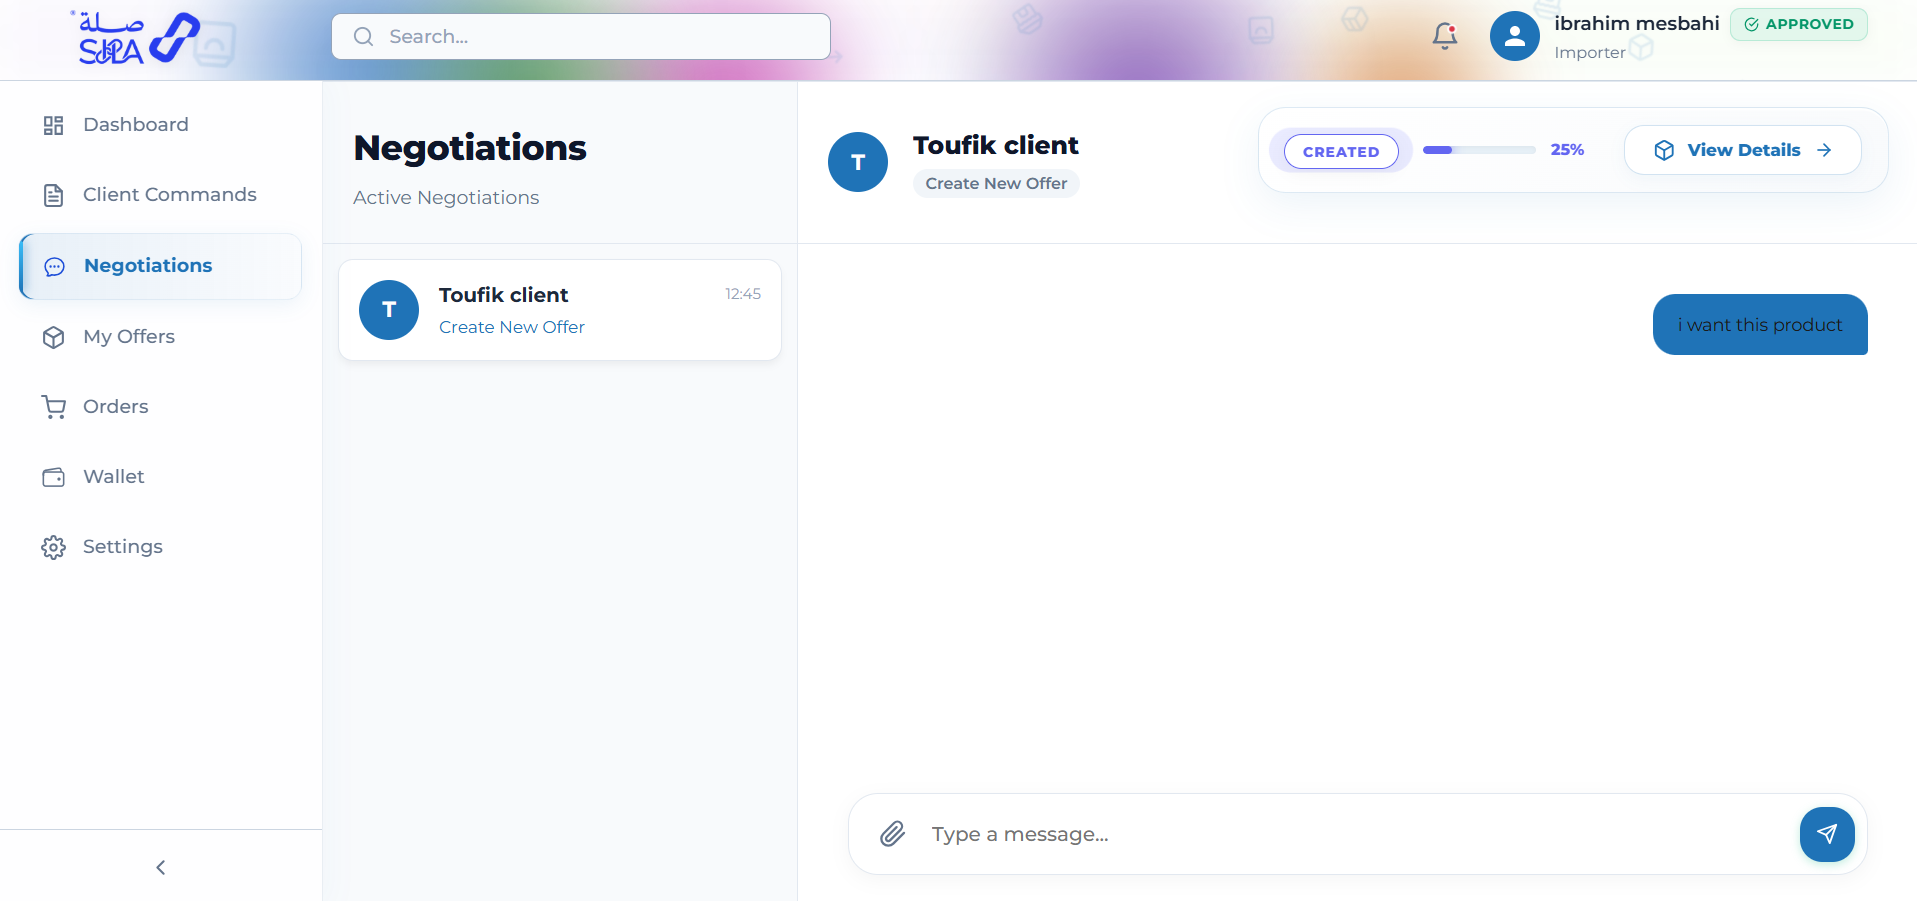
\includegraphics[width=0.9\textwidth]{assets/NEGOCIATION.png}
    \caption{Real-time Negotiation Interface}
    \label{fig:negotiation}
\end{figure}
% ==========================================================

\subsection{Points and Wallet System}
To sustain the business model, the wallet module handles financial tracking. Importers can monitor their subscriptions and purchase points. The backend ensures ACID compliance using PostgreSQL to prevent race conditions during points deduction (e.g., when boosting an offer).

% =========== WALLET SCREENSHOT ===========
\begin{figure}[H]
    \centering
    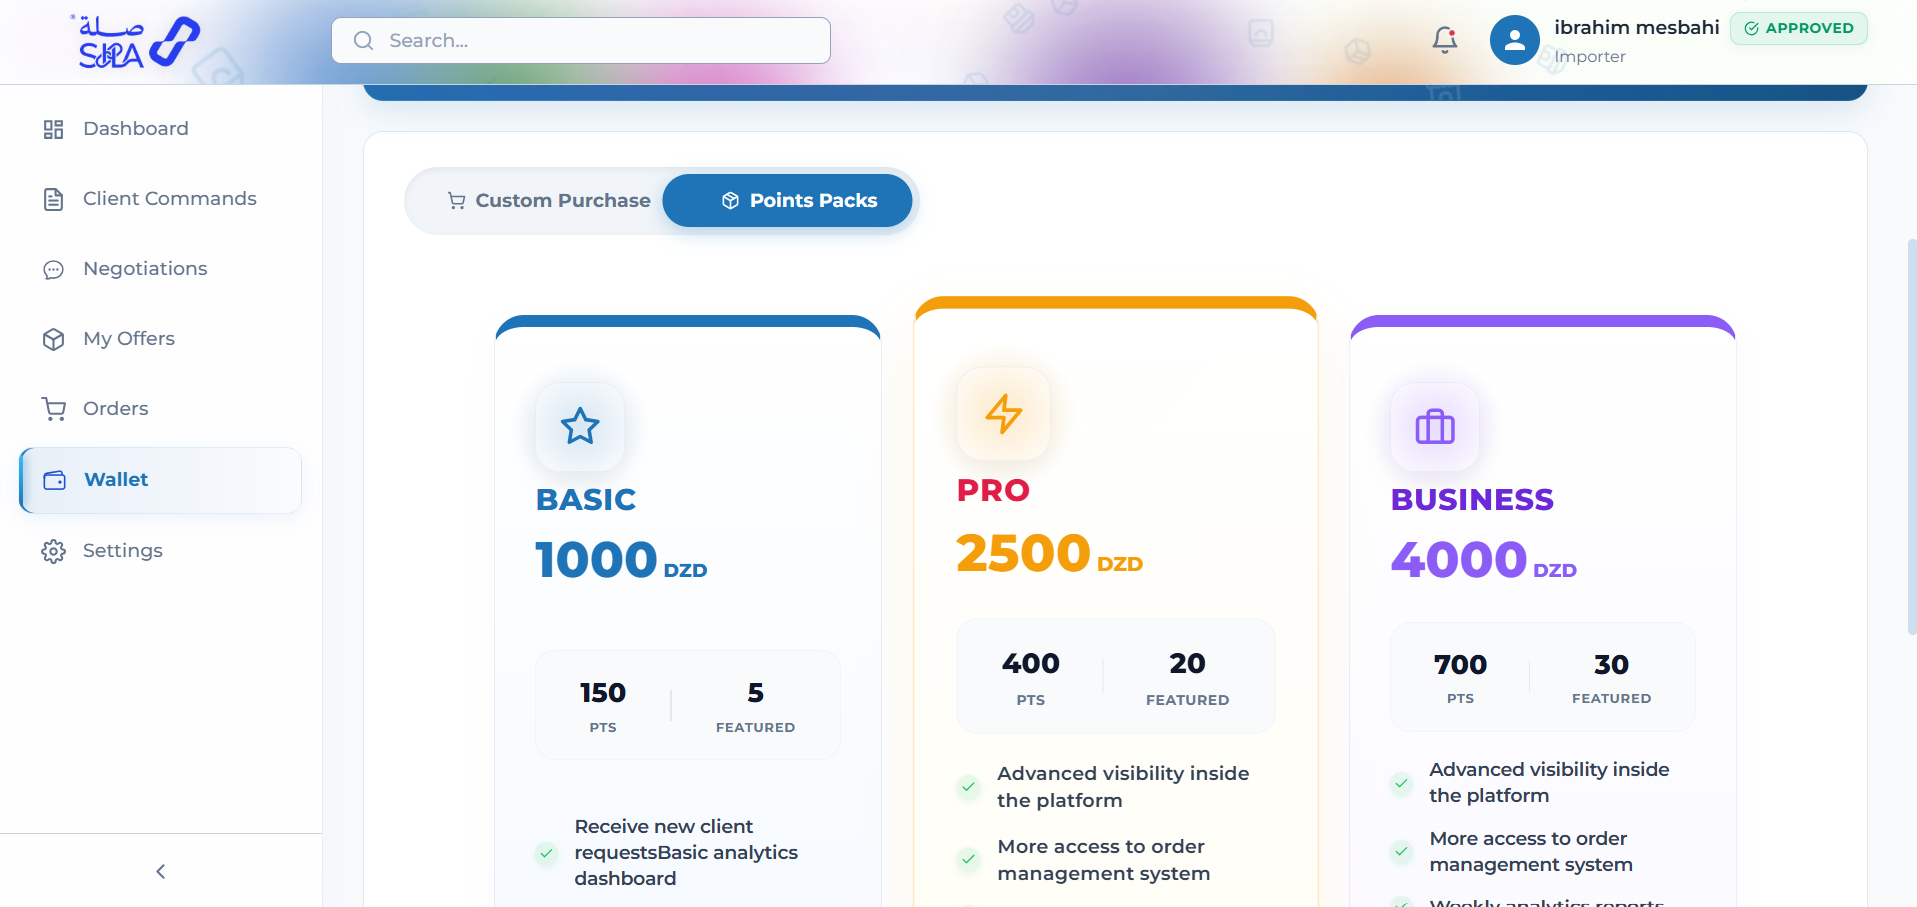
\includegraphics[width=0.9\textwidth]{assets/WALLET.png}
    \caption{Wallet and Points Management Interface}
    \label{fig:wallet}
\end{figure}
% =====================================================
